\chapter {Diseño}

\section{Arquitectura objetivo}
\subsection{Servidores Físicos}
\begin{text}
	Al trabajar en una empresa de hosting, he tenido la suerte de contar con 3 servidores bare metal para el desarrollo de este proyecto. Las características técnicas de los servidores se pueden consultar en \nameref{servidores_bare_metal}.
\end{text}
\subsection{Infraestructura objetivo}
\begin{text}
	Este proyecto pretende crear una infraestructura para una pequeña empresa que se dedique al desarrollo del software. Esta infraestructura debe ser segura, con lo que ha de proporcionar firewalls redundantes y algún mecanismo para proporcional alta disponibilidad en las aplicaciones web.  A continuación se muestra la infraestructura objetivo. Cabe destacar que las Ips y la información que se muestra en la figura es únicamente de este proyecto con los dominios e IPs contratadas. Sin embargo, la red LAN dentro del cluster sí que se mantendría en otros despliegues del cluster, ya que está no depende de servicios externos. La siguiente figura muestra la estructura general de la infraestructura. Sin embargo, es necesario un nivel de abstracción más bajo para conocer los distintos servicios desplegados en el cluster bajo la red \textbf{10.6.0.0/16}.
	
	\clearpage
	
	\begin{figure}[!hbt]
		\label{InfraestructuraObjetivo}
		\centering
		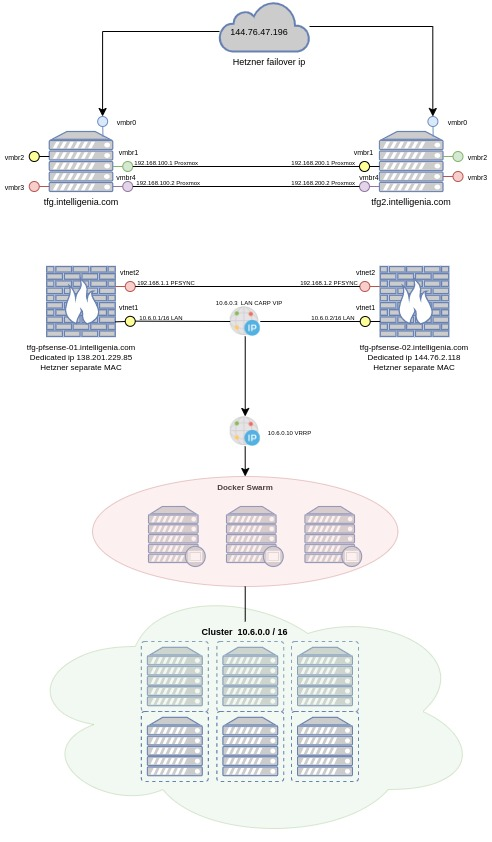
\includegraphics[scale=0.75]{imagenes/Analisis/diagrama.jpg}
		\caption[Infraestructura Objetivo]{Infraestructura Objetivo}
	\end{figure}
\end{text}

\clearpage

\subsection{VSwitch}
\begin{text}
	El cluster está bajo la red LAN 10.6.0.0/16, de forma que todas las máquinas virtuales están comunicadas. Sin embargo los nodos principales (tfg.intelligenia.com, tfg2.intelligenia.com y tfg3.intelligenia.com) tienen que estar comunicados a través de una red interna para el correcto funcionamiento de Proxmox y los pfSense.
	Es aquí donde entran en juego los switches virtuales de Hetzner. Un VSwitch simula el funcionamiento de un switch convencional, conectando los servidores que se conecten al switch entre sí. De este modo, conseguimos crear una red de conexión entre los nodos principales.
	
	\begin{figure}[!hbt]
		\centering
		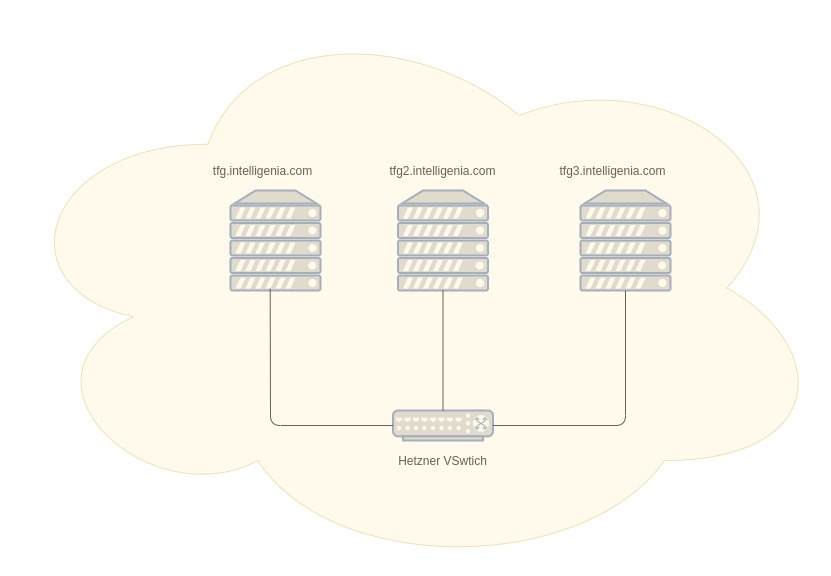
\includegraphics[scale=0.4]{imagenes/Analisis/vswitch.jpg}
		\caption[VSwitch]{VSwitch}
		\label{VSwitch}
	\end{figure}
\end{text}

\begin{text}
	La infraestructura anterior junto con los cauces pertinentes para la integración y despliegues continuos, es lo que pretende este proyecto. A continuación se explica como se ha diseñado la solución que satisface los requisitos funcionales relacionados con lac reación y despliegue de infraestructura con la herramienta de automatización Ansible.
\end{text}
\clearpage

\subsection{Diagrama Cluster}

\begin{text}
	La siguiente figura muestra el cluster con un nivel de abstracción más bajo. Se muestran los distintos servicios que ofrece el cluster y la relación entre ellos. Cada servicio desplegado contribuye a la realización de uno o más requisitos funcionales descritos en la sección \nameref{requisitosfuncionales} cucho propósito es lograr los objetivos definidos en \nameref{subobjetivos}. \\
	El cluster de servicios está interconectado entre sí en la red \textbf{10.6.100.0/24}.
\end{text}
\begin{figure}[!hbt]
	\centering
	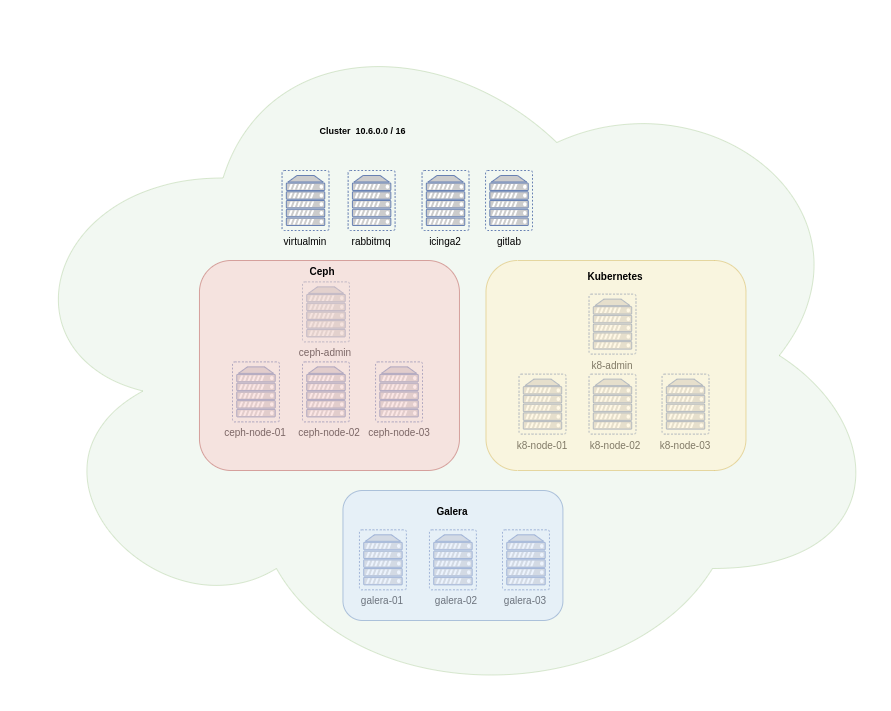
\includegraphics[scale=0.40]{imagenes/Diseno/diagrama_cluster_2.png}
	\caption[Diseño Cluster]{Diseño Cluster} 
	\label{cluster_design}
\end{figure}

\section{Diseño de la solución basado en Ansible}
\begin{text}
	Como se ha discutido en la sección \nameref{tecnologias_elegidas} hemos elegido Ansible para cumplir los objetivos de este proyecto. Ansible nos permite automatizar el proceso de creación y configuración de la infraestructura. En la siguiente sección se hace un análisis de como se ha ido construyendo la solución utilizando Ansible en términos de metodología y forma de estructura el proyecto.
\end{text}

\subsection{Estructura, modularización y metodología}
\begin{text}
	Para diseñar la estructura y la metodología a seguir en el desarrollo se ha partido de los \nameref{requisitosfuncionales}. Para entender la metodología utilizada hay que conocer como funciona Ansible.
	
	\subsubsection{Ansible}
	\label{ansible_}
	\begin{text}
		Ansible es una herramienta de automatización que nos permite lanzar playbooks contra servidores remotos o locales.
		\begin{itemize}
			\item \textbf{Playbooks}: un playbook consiste en un conjunto de tareas que se ejecutan de forma secuencial en los hosts definidos. Sin embargo, los playbooks por si solos aportan poca flexibilidad a la hora de estructurar los proyectos y dificulta la comprensión de estos ya que se pueden convertir en ficheros muy largos difíciles de seguir. Es por esto que surge la necesidad de organizar de algún modo las tareas por funcionalidad. Es aquí donde surgen los roles.
			
			\item \textbf{Roles:}: un role nos permite agrupar múltiples tareas bajo un mismo nombre. Por ejemplo, podríamos crear un role llamado firewall en el cual definiríamos todas las tareas que involucren al firewall. Ésto hace que el proyecto sea más legible y ayuda al futuro desarrollo.
		\end{itemize}
	
	Para cada caso de uso definido en \nameref{casosdeuso} se ha creado un playbook. En nuestro caso, hemos creado un role para cada servicio desplegado en el cluster. Estos roles harán los playbooks más legibles. \\
	En cada role se definen una serie de variables para decidir qué tareas se van a lanzar. Para explicar esto pongamos el ejemplo del role \textbf{webproxy}. Este role tiene varias tareas:
	\begin{itemize}
		\item \textbf{apply\_config.yml}
		\item \textbf{create\_site.yml}
		\item \textbf{create\_ssl\_cert.yml}
		\item \textbf{install\_certbot.yml}
		\item \textbf{install\_nginx.yml}
	\end{itemize}

	Podría darse el caso que quisieramos crear un sitio en nginx sin certificado SSL. Para esto se han definido unas variables que se han de definir en cada playbook para elegir qué tareas lanzar de cada role. \\
	Cada tarea definida en los role, corresponde con un issue definido en \nameref{issues}.
	
	\clearpage
	
	A continuación se listan los distintos playbooks definidos y se relacionan con sus correspondientes \nameref{requisitosfuncionales} e \nameref{issues}.
	
	\begin{itemize}
		\item \textbf{configure\_local\_environment.yml}. \hyperref[RF0]{RF0}.
		\begin{itemize}
			\item Issue 0.1 - 0.2.
		\end{itemize}
	
		\item \textbf{configure\_proxmox\_node.yml}. \hyperref[RF1]{RF1}, \hyperref[RF4]{RF4}.
		\begin{itemize}
			\item Issue 1 - 1.10.
		\end{itemize}
	
		\item \textbf{apply\_config\_pfsense.yml}. \hyperref[RF3]{RF3}, \hyperref[RF4]{RF4}.
		\begin{itemize}
			\item Issue 2.3.
		\end{itemize}
	
		\item \textbf{deploy\_pfsense\_firewall.yml}. \hyperref[RF3]{RF3}, \hyperref[RF4]{RF4}.
		\begin{itemize}
			\item Issue 2.1,2.2,2.4.
		\end{itemize}
		
		\item \textbf{create\_gitlab.yml}. \hyperref[RF3]{RF3}, \hyperref[RF4]{RF4}.
		\begin{itemize}
			\item Issue 3.1 - 3.4.
		\end{itemize}
	
		\item \textbf{create\_ceph\_cluster.yml}. \hyperref[RF3]{RF3}, \hyperref[RF4]{RF4}.
		\begin{itemize}
			\item Issue 5.1.
		\end{itemize}
	
		\item \textbf{create\_virtualmin.yml}. \hyperref[RF3]{RF3}, \hyperref[RF4]{RF4}.
		\begin{itemize}
			\item Issue 5.3.
		\end{itemize}
	
		\item \textbf{create\_webproxy.yml}. \hyperref[RF3]{RF3}, \hyperref[RF4]{RF4}.
		\begin{itemize}
			\item Issue 5.6.
		\end{itemize}
	
		\item \textbf{create\_icinga2.yml}. \hyperref[RF3]{RF3}, \hyperref[RF4]{RF4}.
		\begin{itemize}
			\item Issue 4.1 - 4.4.
		\end{itemize}
	
		\item \textbf{create\_galera\_cluster.yml}. \hyperref[RF3]{RF3}, \hyperref[RF4]{RF4}.
		\begin{itemize}
			\item Issue 5.2.
		\end{itemize}
	
		\item \textbf{create\_rabbitmq.yml}. \hyperref[RF3]{RF3}, \hyperref[RF4]{RF4}.
		\begin{itemize}
			\item Issue 5.5.
		\end{itemize}
	
		\item \textbf{create\_docker\_swarm\_cluster.yml}. \hyperref[RF3]{RF3}, \hyperref[RF4]{RF4}.
		\begin{itemize}
			\item Issue 5.7.
		\end{itemize}
		\item \textbf{create\_kubernetes\_cluster.yml}. \hyperref[RF3]{RF3}, \hyperref[RF4]{RF4}.
		\begin{itemize}
			\item Issue 5.7.
		\end{itemize}
		
	\end{itemize}

	\end{text}
\end{text}

\subsection{Despliegue solución}
\begin{text}
	Una vez diseñada e implementada la solución su despliegue consiste en ejecutar los distintos playbooks en la infraestructura objetivo. Sin embargo, antes de poder lanzar estos playbooks, hay que configurar un fichero \textbf{hosts.yml} donde definimos los hosts donde desplegar el proyecto así como la distribución de servicios en los nodos y otra información como la IP de cada servicio. \\
	Una vez realizada la configuración pertinente, el único requisito por parte de la empresa es el alquiler de 2 o más servidores (bare metal) en Hetzner \cite{hetzner:online}.
\end{text}

\subsection{Cumplimiento requisitos funcionales}
\begin{text}
	Al haber estructurado el proyecto creando un playbook o más por cada requisito funcional, y al tener cada role definidos una serie de test, si se cumple el objetivo de cada playbook, se cumplirán los requisitos funcionales. \\
	Como hemos comentado en la sección \nameref{ansible_}, Ansible se encarga de ejecutar las tareas definidas en los roles y en los playbooks de forma secuencial. Cada tarea de Ansible tiene un objetivo el cual si no se cumple, se lanza una excepción en forma de error abortando la ejecución del playbook. Esta forma de funcionar nos asegura que, si un playbook de los definidos en este proyecto termina su ejecución con éxito, los issues a los que está asociado dicho playbook van a quedar resueltos.
\end{text}

\section{Posibles mejoras}
        \begin{text}
                El proyecto que describe este documento, es una solución integral para resolver el problema de infraestructura en una pequeña empresa. Si hablamos de posibles mejoras, ya que siempre se puede mejorar, hablaríamos de hacer más eficientes los playbooks de Ansible o estructurarlos de forma que sean más comprensibles si cabe. Cabe destacar que en el diseño del cluster se incluye un cluster de Kubernetes, el cual está justamente para mejorar el cluster de docker-swarm. \\
                Un punto importante de mejora sería implementar las técnicas de integración continua y entrega continua a las aplicaciones Wordpress de Virtualmin, ya que en este proyecto únicamente se abordan los proyectos Django + Angular de la empresa. \\
                A grandes rasgos y exceptuando pequeñas mejoras en la calidad del código o la documentación, pienso que el proyecto es muy ambicioso y está bien diseñado a nivel de infraestructura, no necesitando grandes cambios en un futuro próximo.
        \end{text}